\section{Property Graph Matching Framework}\label{sec:framework}
Figure~\ref{img:framework} shows the main execution workflow of our framework.
Basically, the framework contains three parts:
\begin{enumerate*}[label={\arabic*.}]
\item Filter on data graph;
\item Compression of intermediate results;
\item Join on compressed data.
\end{enumerate*}
\begin{figure}[ht]
  \centering
  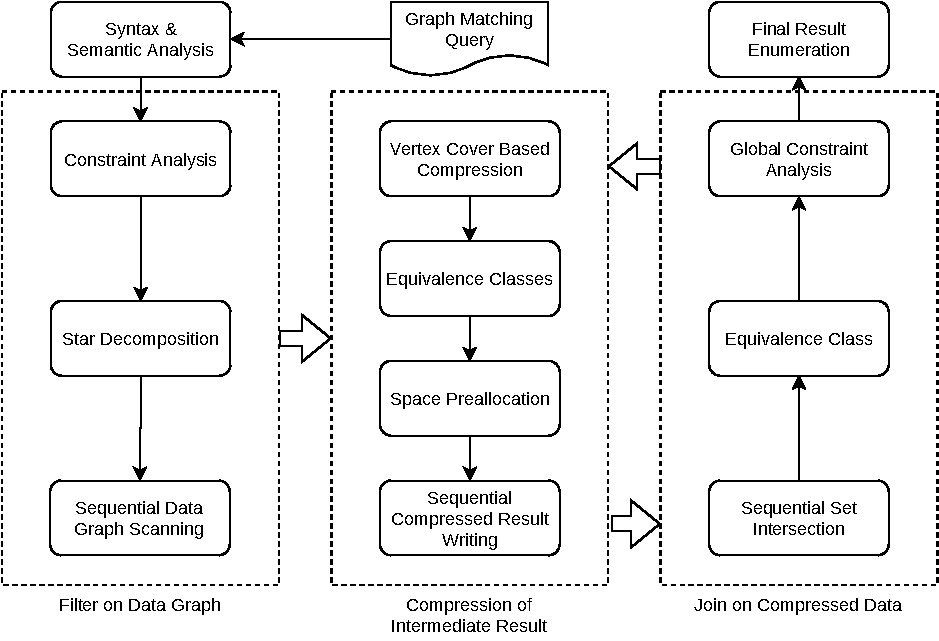
\includegraphics[width=.48\textwidth]{img/framework.pdf}
  \caption{Main Execution Workflow.}\label{img:framework}
\end{figure}
We adopt a join-based method instead of tree-search method to match property graph in an out-of-core environment for two reasons:
Firstly, join-based method is more suitable for real-world graph databases,
the pattern graph is decomposed into smaller parts and matched separately and these partial results can be used as caches for queries afterward;
Secondly, a tree-search method will result in considerable disk I/O because the data vertices are scattered among the disk file.

In order to demonstrate the workflow clearly,
consider the Cypher query in Figure~\ref{img:cypher_query} which corresponds to the pattern graph in Figure~\ref{img:pattern}
(For simplicity, the properties are ignored and use the ID of vertices instead in the WHERE clause).
\begin{figure}[ht]
  \begin{minted}[fontsize=\scriptsize]{cypher}
    MATCH (u1:Person)-[:FOLLOWS]->(u2:Person)-[:FOLLOWS]->(u1),
          (u1)-[:FOLLOWS]->(u3:Person)-[:FOLLOWS]->(u1),
          (u1)-[:PUBLISHES]->(u4:Media), (u1)-[:LIKES]->(u4),
          (u2)-[:LIKES]->(u4)<-[:LIKES]-(u3)
    WHERE id(u1) < id(u2) AND id(u1) < id(u3) AND
          NOT (id(u2) >= id(u3) OR id(u4) >= 2020)
  \end{minted}
  \caption{Graph matching query of the pattern graph in Figure~\ref{img:pattern}.}\label{img:cypher_query}
\end{figure}

\textbf{A graph matching query consists two parts: the pattern graph description part (the MATCH clause) and the constraint specification part (the WHERE clause)}.
It is also possible to support other graph query language if the parser is changed respectively.
The syntax and semantic analyzer would analyze the graph matching query,
check the graph and types, and then generate a valid abstract syntax tree (AST).
Readers interested in these subjects could refer to the textbook~\cite{friedman2001essentials} and we would not discuss it further in this paper.
In the following sections, we will focus on the three main stages of our property graph matching system (as shown in Figure~\ref{img:framework}).

Section~\ref{sec:filter_on_data_graph} describes the first filtering stage, in which we try to reduce not only the output size of the intermediate results,
but also the input size by reading only necessary parts from the huge data graph file.
This is achieved by \textbf{a properly decomposition} of both the constraint specification part (Section~\ref{sec:constraint_analysis})
and the graph description part (Section~\ref{sec:star_decomposition}) of the query,
which is distinct from previous works that our method will hold all structural information that can be used to minimize the disk I/O.
We also design an efficient disk-based \textbf{graph index} (Section~\ref{sec:data_graph_scanning}), such that only one sequential read of the origianl
graph is needed to match all the decomposed atomic query and the preserved structural information
can be used to skip unnecessary parts of the graph.

In Section~\ref{sec:compression_of_intermediate_result}, we demonstrate the data structure that we use to express the intermediate results of graph matching
\textbf{with an extremly high compression ratio}.
Our compression algorithm is based on VCBC~\cite{DBLP:journals/pvldb/QiaoZC17}, and we will give a brief review of the VCBC algorithm in Section~\ref{sec:vcbc}.
To reduce the I/O cost even further, in Section~\ref{sec:equivalence_classes}, we study the \emph{NeighborInfo equivalence classes} in the pattern graphs and use
these equivalence classes to avoid blindly matching result writing. To put theory into practice, one more challenge
is how to write this compressed expression to file without introducing random disk I/O.
To solve this problem, we propose a space pre-allocation method in Section~\ref{sec:space_allocation}.

Finally, Section~\ref{sec:join_on_compressed_data} provides how we join the compressed intermediate results to obtain the
final matching results. To reduce the I/O cost, our algorithm is elegantly designed such that the set intersection
operation could be performed sequentially in linear time (Section~\ref{sec:sequential_set_intersection}).
The space allocation problem still occurred during the join phase, in Section~\ref{sec:space_allocation_eqv} we will address this problem,
and we will show that the equivalence classes can still be applied here to reduce I/O cost further.
At last, in Section~\ref{sec:global_constraint_analysis}, we will describe how to boost the join operation by the user-provided searching conditions.
